\chapter{量子数与电子排布}\label{ch:b1:quantum-numbers}

在低压下向玻璃管中充入氢气，并通电放电，
透过棱镜观察发出的粉红色辉光。
这种光并未展开成彩虹，而是分裂为四条清晰的谱线——
一条红色、一条蓝绿色、两条紫色——谱线之间别无他光。热的固体在每个波长上都发光；
而氢原子只发出少数几条谱线。
这一解释形成于 1913 至 1926 年间：原子中电子的能量
不能取任意值，它是\emph{量子化的}。本章按化学家的用法
叙述这种量子化的规则——四个量子数、三条填充规则——
并由此得出每个原子和离子的
电子排布，它是
下一章元素周期表的关键。

\begin{recall}
第 1 册（十年级）介绍了前二十号元素的电子在
电子层和电子亚层中的排布，即 1s、2s、2p、3s、3p，
并称最外层电子为价电子。由物理学已知，
波长为 $\lambda$ 的光由能量为
$E = h\nu = hc/\lambda$ 的光子组成，
其中 $h$ 为普朗克常量，$c$ 为光速。
\end{recall}

\begin{omfigure}

\includegraphics[width=0.62\linewidth]{images/book2/ai/b1-01-street-lamps.jpg}

{\small 低压钠灯。它的光几乎是单一的
橙黄色谱线：与氢一样，受激的钠原子只发出
少数几种确定能量的光子。}
\end{omfigure}

\section{量子化的能量：氢原子光谱}

\begin{definition}[能级、基态与激发态]\label{def:b1:quantum-numbers:energy-level}
原子中束缚电子的能量只能取
某些特定值，这些值称为原子的\emph{能级}\index{能级}。
能量零点取为电子静止于距原子核无穷远处时的能量，
此时原子已被电离，因此束缚电子的各能级均为负值。
最低的能级称为\emph{基态}\index{基态}；
其余各能级都称为\emph{激发态}\index{激发态}。
\end{definition}

原子从能量为 $E_{\text{高}}$ 的能级跃迁到较低能级
$E_{\text{低}}$ 时放出一个光子；反之，由较低能级跃迁到较高能级时，
则吸收一个能量为下式的光子：
\[
  h\nu = \frac{hc}{\lambda} = E_{\text{高}} - E_{\text{低}} .
\]
因此，谱线光谱反映的是
各能级之间的能量差。

\begin{theorem}[氢原子的能级]\label{thm:b1:quantum-numbers:levels}
氢原子的能级为
\[
  E_n = -\frac{E_R}{n^2}, \qquad n = 1, 2, 3, \dots,
  \qquad E_R = \qty{13.6}{eV},
\]
其中 $E_R$ 为里德伯能量（已对原子核的
运动作了修正）。基态能级为 $E_1 = \qty{-13.6}{eV}$，原子的
电离能为 $E_R$。
% ledger: const:RyhcEV, ie:H (13.598 eV; levels computed in
% figdata/bachelor-1/hydrogen-levels.py)
\end{theorem}
\admitted

\begin{remark}[公式的来源]\label{rem:b1:quantum-numbers:schrodinger}
该公式由求解电子在质子场中的薛定谔方程得出；
其解以及由此给出的波函数形状，
在本科二年级分册中推导。玻尔曾于 1913 年
由一个更简单的圆轨道模型得到相同的能级，
该模型现已被弃用。
\end{remark}

\begin{proposition}[里德伯公式]\label{prop:b1:quantum-numbers:rydberg}
氢原子发出的谱线，其波长由下式给出：
\[
  \frac{1}{\lambda} = R_H\left(\frac{1}{n_1^2} - \frac{1}{n_2^2}\right),
  \qquad n_2 > n_1 \ge 1, \qquad R_H = \frac{E_R}{hc},
\]
对应于从能级 $n_2$ 跃迁到能级 $n_1$ 的情形。终止于同一能级 $n_1$ 的谱线
构成一个\emph{线系}：$n_1 = 1$ 为莱曼系（紫外），
$n_1 = 2$ 为巴耳末系（可见光），$n_1 = 3$ 为帕邢系
（红外）。
\end{proposition}

\begin{proof}
光子带走了原子失去的能量：
$hc/\lambda = E_{n_2} - E_{n_1} = -E_R/n_2^2 + E_R/n_1^2
= E_R\,(1/n_1^2 - 1/n_2^2)$。两边除以 $hc$ 即得公式。
\end{proof}

\begin{example}[氢的红色谱线]\label{ex:b1:quantum-numbers:halpha}
对于跃迁 $3 \to 2$：$\Delta E = 13.6\,(1/4 - 1/9) =
\qty{1.89}{eV}$。取 $hc = \qty{1240}{eV.nm}$（由 $h$，
$c$ 和 $e$ 的值得出），$\lambda = 1240/1.89 = \qty{656}{nm}$：红色谱线。
其余巴耳末系谱线 $4 \to 2$、$5 \to 2$、$6 \to 2$ 分别位于 486、
434 和 \qty{410}{nm}；下一条 $7 \to 2$ 位于 \qty{397}{nm}，
已处于紫外区。实测波长为 656.3、486.1、434.0
及 \qty{410.2}{nm}，两者符合程度优于二千分之一；
剩余的微小差距源于测量是在空气而非真空中进行的。
% ledger: asd:Halpha, asd:Hbeta, asd:Hgamma, asd:Hdelta (computed values
% in figdata/out/bachelor-1-hydrogen-levels-balmer.dat)
\end{example}

\begin{omfigure}
\begin{tikzpicture}
\begin{axis}[
  width=0.62\linewidth, height=7.2cm,
  xmin=0, xmax=10, ymin=-14.5, ymax=0.6,
  axis x line=none, axis y line=left,
  ylabel={能量 (eV)}, ytick={-14,-12,-10,-8,-6,-4,-2,0},
  tick label style={font=\small}, label style={font=\small},
  clip=false]
\pgfplotsinvokeforeach{-13.598,-3.400,-1.511,-0.850,-0.544}{
  \draw[black!70, line width=0.7pt] (axis cs:0.3,#1) -- (axis cs:9.6,#1);}
\draw[black!40, dashed] (axis cs:0.3,0) -- (axis cs:9.6,0);
\node[font=\small, anchor=west] at (axis cs:9.7,-13.598) {$n = 1$};
\node[font=\small, anchor=west] at (axis cs:9.7,-3.400) {$n = 2$};
\node[font=\small, anchor=west] at (axis cs:9.7,-1.511) {$n = 3$};
\node[font=\small, anchor=south west] at (axis cs:9.7,0.05) {$n \to \infty$};
% Lyman
\draw[-{Stealth}, violet!70!black, thick] (axis cs:1.0,-3.400) -- (axis cs:1.0,-13.598);
\draw[-{Stealth}, violet!70!black, thick] (axis cs:1.6,-1.511) -- (axis cs:1.6,-13.598);
\draw[-{Stealth}, violet!70!black, thick] (axis cs:2.2,-0.850) -- (axis cs:2.2,-13.598);
\node[font=\small, violet!70!black, anchor=west] at (axis cs:2.4,-9) {莱曼};
% Balmer
\draw[-{Stealth}, red!80!black, thick] (axis cs:4.4,-1.511) -- (axis cs:4.4,-3.400);
\draw[-{Stealth}, teal!80!black, thick] (axis cs:5.0,-0.850) -- (axis cs:5.0,-3.400);
\draw[-{Stealth}, blue!80!black, thick] (axis cs:5.6,-0.544) -- (axis cs:5.6,-3.400);
\node[font=\small, anchor=north] at (axis cs:5.0,-3.6) {巴耳末};
% Paschen
\draw[-{Stealth}, black!60, thick] (axis cs:7.8,-0.850) -- (axis cs:7.8,-1.511);
\draw[-{Stealth}, black!60, thick] (axis cs:8.4,-0.544) -- (axis cs:8.4,-1.511);
\node[font=\small, anchor=north] at (axis cs:8.1,-1.7) {帕邢};
\end{axis}
\end{tikzpicture}

{\small 氢原子的能级 $E_n = -\qty{13.6}{eV}/n^2$，
按比例绘制（由里德伯常量算得）；能级 $n = 4,
5, \dots$ 挤在零以下。每个箭头表示一个
所发射的光子；终点相同的箭头构成一个谱线系。}
\end{omfigure}

\begin{omfigure}
\begin{tikzpicture}
\begin{axis}[
  width=0.9\linewidth, height=3.0cm,
  xmin=360, xmax=700, ymin=0, ymax=1,
  axis x line=bottom, axis y line=none,
  xlabel={波长 (nm)}, xtick={400,450,500,550,600,650,700},
  tick label style={font=\small}, label style={font=\small},
  clip=false]
\fill[black!85] (axis cs:360,0) rectangle (axis cs:700,1);
% line positions: figdata/out/bachelor-1-hydrogen-levels-balmer.dat
\draw[line width=1.6pt, red!90!black] (axis cs:656.5,0) -- (axis cs:656.5,1);
\draw[line width=1.6pt, cyan!80!green] (axis cs:486.3,0) -- (axis cs:486.3,1);
\draw[line width=1.6pt, blue!70!violet] (axis cs:434.2,0) -- (axis cs:434.2,1);
\draw[line width=1.6pt, violet!75] (axis cs:410.3,0) -- (axis cs:410.3,1);
\draw[white, dashed] (axis cs:364.7,0) -- (axis cs:364.7,1);
\node[font=\small, anchor=south] at (axis cs:364.7,1.02) {极限};
\node[font=\small, anchor=south] at (axis cs:656.5,1.02) {$3\to2$};
\node[font=\small, anchor=south] at (axis cs:486.3,1.02) {$4\to2$};
\node[font=\small, anchor=south] at (axis cs:434.2,1.02) {$5\to2$};
\node[font=\small, anchor=south east] at (axis cs:412,1.02) {$6\to2$};
\end{axis}
\end{tikzpicture}

{\small 由里德伯公式算得的巴耳末谱线（真空
波长），位于可见光波段。更多谱线向线系
极限 \qty{364.7}{nm} 处密集，位于紫外线区域。}
\end{omfigure}

\begin{history}[玻尔的原子模型，1913]
1913 年，年仅 28 岁、在曼彻斯特工作的丹麦物理学家尼尔斯·玻尔
提出：氢原子的电子只能绕原子核在某些
特定轨道上运动，电子从一条轨道
跃迁到较低轨道时发出光。他的模型精确给出了巴耳末线，以及
里德伯常量的值（由 $h$、$e$ 和电子质量得到）。
这些轨道概念未能经受住 1925--1926 年量子力学的检验，但
量子化的能级却被保留了下来。玻尔于 1922 年获得诺贝尔物理学奖。
\end{history}

\begin{omfigure}
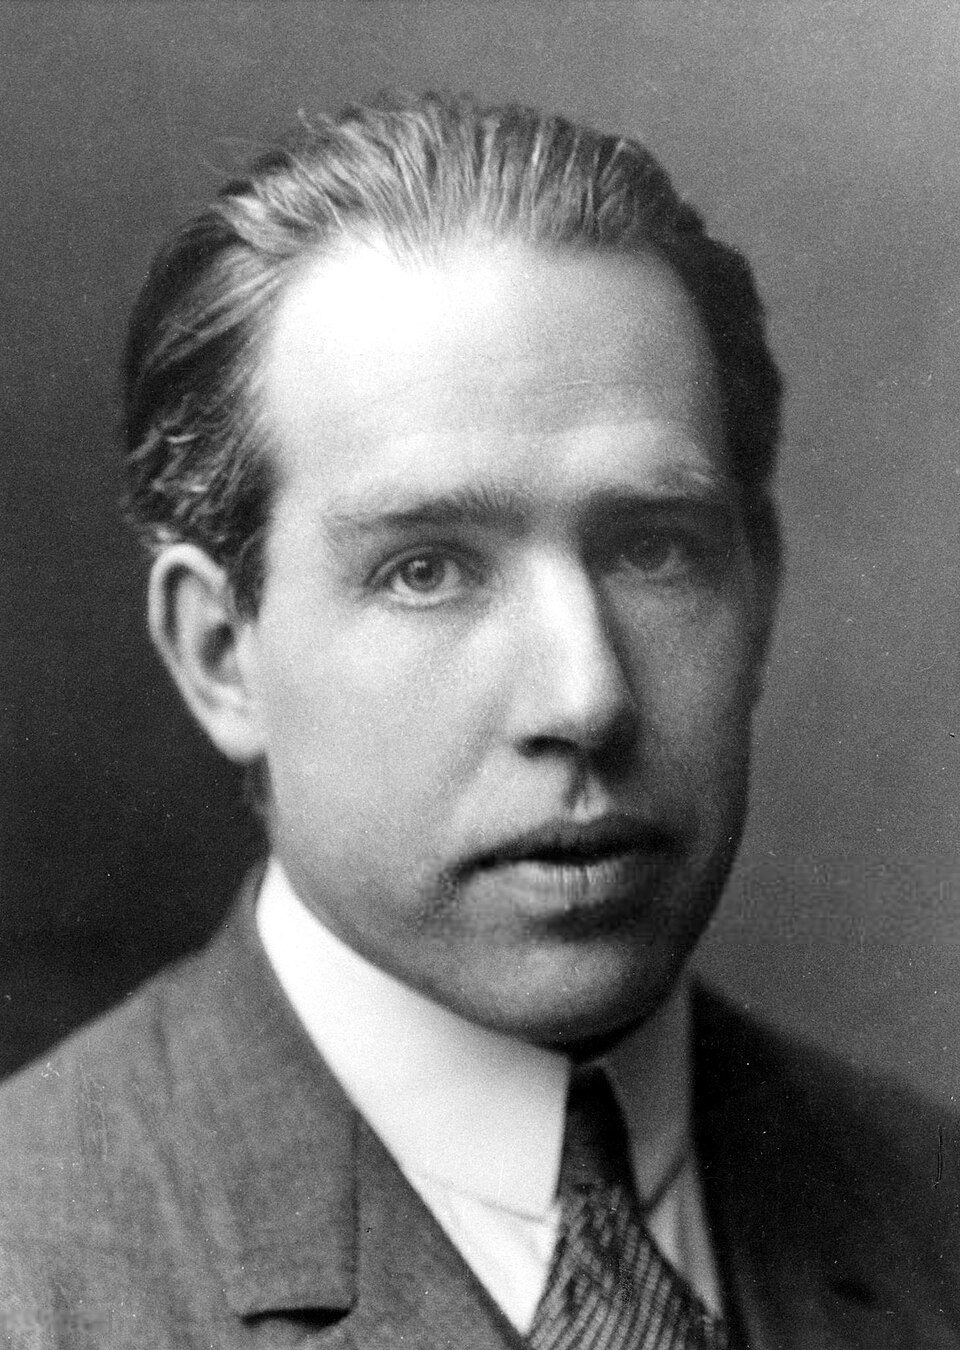
\includegraphics[width=0.26\linewidth]{images/book2/bohr.jpg}

{\small 尼尔斯·玻尔（1885--1962），约摄于 1922 年。}
\end{omfigure}

\section{四个量子数}

在多电子原子中，能量不再由一个
简单公式给出，但每个电子仍由一组少量
整数描述，即它的量子数。

\begin{definition}[量子数]\label{def:b1:quantum-numbers:quantum-number}
原子中电子的状态由四个数标记：
\begin{itemize}
  \item \emph{主量子数}\index{主量子数}
        $n = 1, 2, 3, \dots$，主要决定能量和大小；
  \item \emph{角量子数}\index{角量子数}
        （或称副量子数）$l = 0, 1, \dots, n-1$，决定
        形状；$l = 0, 1, 2, 3$ 分别记为 s、p、d、f；
  \item \emph{磁量子数}\index{磁量子数}
        $m_l = -l, -l+1, \dots, l$，决定取向（$2l + 1$
        个取值）；
  \item \emph{自旋量子数}\index{自旋量子数}
        $m_s = +\tfrac12$ 或 $-\tfrac12$，是电子的
        固有性质，用向上或向下的箭头表示。
\end{itemize}
\end{definition}

\begin{definition}[原子轨道、电子层、电子亚层]\label{def:b1:quantum-numbers:orbital}
\emph{原子轨道}\index{原子轨道}是单电子态；
它由三个数 $(n, l, m_l)$ 标记，画成一个方框，
\omorbs{}。具有相同 $n$ 的轨道构成一个\emph{电子
层}\index{电子层}；具有相同 $n$ 和 $l$ 的轨道构成一个
\emph{电子亚层}\index{电子亚层}，以 $n$ 和 $l$ 对应的字母命名：
2p 即 $n = 2$、$l = 1$ 的电子亚层，由三个轨道组成
（$m_l = -1, 0, 1$）。
\end{definition}

\begin{remark}[形状]\label{rem:b1:quantum-numbers:shapes}
s 轨道是球形的；p 轨道沿某一轴有两个瓣，
而三个 2p 轨道分别指向 $x$、$y$ 和 $z$ 方向。这些形状的数学
描述——波函数、其径向与角向部分、
其节点——属于本科二年级分册。在本书中，
轨道是一个最多容纳两个电子的方框。
\end{remark}

\begin{proposition}[电子亚层与电子层的容量]\label{prop:b1:quantum-numbers:capacity}
角量子数为 $l$ 的电子亚层含有 $2l + 1$ 个轨道，最多可容纳
$2(2l + 1)$ 个电子：s 亚层 2 个、p 亚层 6 个、d 亚层 10 个、f 亚层 14 个。电子层 $n$
含有 $n^2$ 个轨道，最多可容纳 $2n^2$ 个电子。
\end{proposition}

\begin{proof}
对给定的 $l$，$m_l$ 取 $2l + 1$ 个值，即从 $-l$ 到 $l$，
每个轨道容纳两个自旋相反的电子（见下文\cref{prop:b1:quantum-numbers:pauli}
）。对给定的 $n$，$l$ 取 $0$ 至 $n - 1$，因此
轨道数为
\[
  \sum_{l=0}^{n-1} (2l+1) = 2\,\frac{(n-1)n}{2} + n = n^2 ,
\]
电子数为 $2n^2$：$n = 1$ 至 4 时分别为 2、8、18、32。
\end{proof}

\begin{example}[第三电子层]\label{ex:b1:quantum-numbers:third}
当 $n = 3$ 时：$l = 0$（3s，一个轨道），$l = 1$（3p，三个轨道），
$l = 2$（3d，五个轨道，$m_l = -2, \dots, 2$）：共九个轨道，至多
可容纳 18 个电子。例如，3d 中某个电子的
量子数为 $(3, 2, -1, +\tfrac12)$。
\end{example}

\section{构建电子排布}

\begin{definition}[电子排布]\label{def:b1:quantum-numbers:configuration}
原子或离子的\emph{电子排布}\index{电子排布}是其占据的各电子亚层及每个亚层中的
电子数组成的列表，以指数形式书写：
氧的电子排布为 $1\text{s}^2 2\text{s}^2
2\text{p}^4$。最高 $n$ 的电子，
连同未填满的 d 或 f 亚层中的电子，是\emph{价
电子}\index{价电子}；其余电子是\emph{内
层电子}\index{内层电子}。书写电子排布时，可
将前一稀有气体的电子排布写在方括号内以简写：
氧为 $[\ce{He}]\,2\text{s}^2 2\text{p}^4$。
\end{definition}

基态电子排布由以下三条规则确定。

\begin{proposition}[泡利不相容原理]\label{prop:b1:quantum-numbers:pauli}
同一原子中，没有两个电子具有完全相同的四个量子数。
因此，一个轨道至多容纳两个电子，
且二者自旋相反：\omorbs{ud}。
\end{proposition}
\admitted

\begin{proposition}[克氏规则]\label{prop:b1:quantum-numbers:klechkowski}
在中性原子的基态中，电子亚层按
$n + l$ 递增的顺序填充；对于相同的 $n + l$，按
$n$ 递增的顺序填充：
\[
  1\text{s},\ 2\text{s},\ 2\text{p},\ 3\text{s},\ 3\text{p},\ 4\text{s},\
  3\text{d},\ 4\text{p},\ 5\text{s},\ 4\text{d},\ 5\text{p},\ 6\text{s},\
  4\text{f},\ 5\text{d},\ 6\text{p},\ 7\text{s},\ 5\text{f},\ 6\text{d},\
  7\text{p}.
\]
\end{proposition}
\admitted

\begin{remark}[经验规则]\label{rem:b1:quantum-numbers:klech-empirical}
克氏规则（亦称马德隆规则）是对观测到的电子排布的总结，
而非定律：它描述了随核电荷增加，电子亚层的填充顺序。
在电子数众多的原子中，电子彼此排斥，因此
亚层的能量
不仅取决于 $l$，也取决于 $n$：一个 4s 电子有一部分时间靠近原子核，
因而在钾和钙中，其能量低于 3d。
\end{remark}

\begin{omfigure}
\begin{tikzpicture}[font=\small, x=1.25cm, y=0.72cm]
  \foreach \n in {1,...,7} {
    \foreach \l/\s in {0/s,1/p,2/d,3/f} {
      \pgfmathtruncatemacro\ok{(\l<\n) && (\n+\l<=8)}
      \ifnum\ok=1
        \node[draw=black!50, rounded corners=2pt, minimum width=0.85cm,
          minimum height=0.5cm, fill=white] (s\n\l) at (\l,-\n) {\n\s};
      \fi
    }
  }
  \begin{scope}[on background layer]
  \foreach \la/\na/\lb/\nb in {0/1/0/1, 0/2/0/2, 1/2/0/3, 1/3/0/4, 2/3/0/5,
      2/4/0/6, 3/4/0/7, 3/5/1/7} {
    \draw[-{Stealth}, omDef, thick, opacity=0.8]
      ($(\la,-\na)+(0.5,0.42)$) -- ($(\lb,-\nb)+(-0.5,-0.42)$);
  }
  \end{scope}
  \node[anchor=west, align=left, font=\small] at (4.0,-2.5) {沿每个箭头走，\\然后走其右侧的下一个 \\箭头};
\end{tikzpicture}

{\small 克氏图。具有相同 $n + l$ 的亚层位于同一条对角线上；
按对角线的顺序依次走，即得填充顺序
1s, 2s, 2p, 3s, 3p, 4s, 3d, 4p, 5s, \dots}
\end{omfigure}

\begin{proposition}[洪特规则]\label{prop:b1:quantum-numbers:hund}
当一个亚层的电子可以放入若干个能量相同的轨道时，
基态具有数目最多的
\emph{平行}自旋：电子先各占一个轨道，自旋均向上，
然后才有轨道被占满两个电子。
\end{proposition}
\admitted

\begin{definition}[未成对电子]\label{def:b1:quantum-numbers:unpaired}
\emph{未成对电子}\index{未成对电子}是单独占据一个轨道的电子。
含有未成对电子的物种会被
磁铁吸引（它具有顺磁性，这是物理学中研究的性质）。
\end{definition}

\begin{method}[书写基态电子排布]\label{met:b1:quantum-numbers:configuration}
要书写原子序数为 $Z$ 的原子的电子排布：
\begin{enumerate}
  \item 按克氏顺序将 $Z$ 个电子填入各亚层，
        每个亚层先填满（容纳 2、6、10、14 个电子）后再填下一个；
  \item 按 $n$ 递增的顺序书写结果（将 3d
        与 $n = 3$ 归为一组），并用前一稀有气体的
        电子排布作为原子实进行简写；
  \item 对于最后一个未填满的亚层，画出轨道框，
        并应用洪特规则统计未成对电子数。
\end{enumerate}
\end{method}

\begin{example}[碳、氮、氧、铁]\label{ex:b1:quantum-numbers:examples}
应用该方法，得到四种原子的结果：
\begin{center}
\begin{tabular}{lllc}
\hline
原子 & 电子排布 & 最后一个亚层 & 未成对电子数 \\
\hline
\ce{C} ($Z = 6$) & $[\ce{He}]\,2\text{s}^2 2\text{p}^2$ & 2p: \omorbs{u,u,} & 2 \\
\ce{N} ($Z = 7$) & $[\ce{He}]\,2\text{s}^2 2\text{p}^3$ & 2p: \omorbs{u,u,u} & 3 \\
\ce{O} ($Z = 8$) & $[\ce{He}]\,2\text{s}^2 2\text{p}^4$ & 2p: \omorbs{ud,u,u} & 2 \\
\ce{Fe} ($Z = 26$) & $[\ce{Ar}]\,3\text{d}^6 4\text{s}^2$ & 3d: \omorbs{ud,u,u,u,u} & 4 \\
\hline
\end{tabular}
\end{center}
对于铁，克氏顺序先填充 4s（$Z = 19, 20$），然后才是 3d
（$Z = 21$ 至 30）；电子排布按 3d 在前的方式书写。
% ledger: gs:Fe
\end{example}

\begin{omfigure}
\begin{tikzpicture}[font=\small]
  \begin{scope}
    \node[anchor=west] at (0,2.4) {\ce{N}: $1\text{s}^2 2\text{s}^2 2\text{p}^3$};
    \node at (0.5,1.3) {\omorbs{ud}}; \node[below] at (0.5,0.9) {1s};
    \node at (1.6,1.3) {\omorbs{ud}}; \node[below] at (1.6,0.9) {2s};
    \node at (3.1,1.3) {\omorbs{u,u,u}}; \node[below] at (3.1,0.9) {2p};
  \end{scope}
  \begin{scope}[xshift=6.2cm]
    \node[anchor=west] at (0,2.4) {\ce{Cr}: $[\ce{Ar}]\,3\text{d}^5 4\text{s}^1$};
    \node at (1.6,1.3) {\omorbs{u,u,u,u,u}}; \node[below] at (1.6,0.9) {3d};
    \node at (4.0,1.3) {\omorbs{u}}; \node[below] at (4.0,0.9) {4s};
    \node[anchor=west, text width=5.0cm] at (0,-0.1) {观察到：六个未成对电子，而非 $3\text{d}^4 4\text{s}^2$};
  \end{scope}
\end{tikzpicture}

{\small 量子格。每个方框代表一个轨道，箭头代表一个电子及其自旋。
氮遵循洪特规则；铬是
\cref{prop:b1:quantum-numbers:exceptions}中的例外之一。}
\end{omfigure}

\section{离子、例外与周期表的形状}

\begin{proposition}[离子的电子排布]\label{prop:b1:quantum-numbers:ions}
单原子阴离子的电子排布，等于原子的电子排布，多出的电子按克氏顺序依次加入；
主族元素的阳离子失去
$n$ 最大的电子。过渡金属的阳离子
则\emph{先}失去 $n$s 电子，然后才失去
$(n-1)$d 电子：\ce{Fe^{2+}} 为 $[\ce{Ar}]\,3\text{d}^6$，
\ce{Fe^{3+}} 为 $[\ce{Ar}]\,3\text{d}^5$，而非 $[\ce{Ar}]\,3\text{d}^4
4\text{s}^2$。
% ledger: gs:Fe2+, gs:Fe3+
\end{proposition}
\admitted

\begin{remark}[填充顺序不等于失去顺序]\label{rem:b1:quantum-numbers:order}
钾和钙中，4s 先于 3d 被填充，但在过渡金属离子中
它却最先被失去。这并不矛盾：亚层能量的次序随核电荷数和电子数而变化，
在过渡金属的原子或离子中，3d 亚层
的能量低于 4s。
克氏规则只适用于中性原子。
\end{remark}

\begin{proposition}[第一过渡系中的两个例外]\label{prop:b1:quantum-numbers:exceptions}
铬和铜的实测基态电子排布为
\[
  \ce{Cr}: [\ce{Ar}]\,3\text{d}^5 4\text{s}^1, \qquad
  \ce{Cu}: [\ce{Ar}]\,3\text{d}^{10} 4\text{s}^1 ,
\]
而非克氏规则预言的 $3\text{d}^4 4\text{s}^2$ 和 $3\text{d}^9 4\text{s}^2$，
半充满或全充满的 d 亚层特别稳定，
而且 4s 与 3d 能级很接近。
% ledger: gs:Cr, gs:Cu
\end{proposition}

\begin{example}[铜及其离子]\label{ex:b1:quantum-numbers:copper}
\ce{Cu} 为 $[\ce{Ar}]\,3\text{d}^{10} 4\text{s}^1$；\ce{Cu+} 为
$[\ce{Ar}]\,3\text{d}^{10}$，没有未成对电子；\ce{Cu^{2+}} 为
$[\ce{Ar}]\,3\text{d}^9$，有一个未成对电子。\ce{Zn^{2+}}，$[\ce{Ar}]\,3\text{d}^{10}$，
没有未成对电子。
% ledger: gs:Cu+, gs:Cu2+, gs:Zn2+
\end{example}

\begin{proposition}[电子排布与周期表]\label{prop:b1:quantum-numbers:table}
周期表的第 $n$ 周期始于 $n$s 亚层的填充，终于 $n$p 亚层的填充。
其间填充的亚层按克氏规则依次为
$(n-2)$f 和 $(n-1)$d。因此各周期容纳
$2, 8, 8, 18, 18, 32, 32$ 种元素，稀有气体的 $Z = 2, 10,
18, 36, 54, 86, 118$。
\end{proposition}

\begin{proof}
第 1 至 3 周期只含 $n$s（$n$p 仅在 $n \ge 2$ 时出现）：先为 $2$，然后
两次 $2 + 6 = 8$。第 4、5 周期加入 $(n-1)$d：$2 + 10 + 6 =
18$。第 6、7 周期还加入 $(n-2)$f：$2 + 14 + 10 + 6 = 32$。稀有气体
封闭每个周期：$2$，$2 + 8 = 10$，$18$，$18 + 18 = 36$，
$54$，$54 + 32 = 86$，$118$。
\end{proof}

\begin{omfigure}
\omperiodictable[colour=blocks, legend]

{\small 按最后被填充亚层着色的周期表：s、p、d 和 f 区。
每个区的宽度即其亚层的容量。
亚层容量依次为 2、6、10 和 14。}
\end{omfigure}

\section{练习}

\begin{exercise}[$\star$]\label{exo:b1:quantum-numbers:1}
下列哪些 $(n, l, m_l, m_s)$ 组可以描述原子中的电子？
逐一说明不可取的理由。
(a) $(2, 2, 0, +\tfrac12)$; (b) $(3, 1, -1, -\tfrac12)$;
(c) $(1, 0, 0, 0)$; (d) $(4, 3, -3, +\tfrac12)$; (e) $(3, 0, 1, -\tfrac12)$.
\end{exercise}

\begin{exercise}[$\star$]\label{exo:b1:quantum-numbers:2}
3d、4f、5p 亚层以及 $n = 2$ 的电子层中，分别有多少个轨道，
最多各能容纳多少个电子？
\end{exercise}

\begin{exercise}[$\star$]\label{exo:b1:quantum-numbers:3}
写出 \ce{O}、\ce{P}、\ce{K}、\ce{Ca}
和 \ce{Br}（$Z = 8, 15, 19, 20, 35$）的基态电子排布，分别用完整形式和简写形式表示，
并给出各自的价电子数。
\end{exercise}

\begin{exercise}[$\star$]\label{exo:b1:quantum-numbers:4}
画出氮、硫和氯的价亚层的量子格，
并数出各自的未成对电子数。
\end{exercise}

\begin{exercise}[$\star\star$]\label{exo:b1:quantum-numbers:5}
写出 \ce{Na+}、\ce{Mg^{2+}}、\ce{Al^{3+}}、\ce{F-}、
\ce{O^{2-}}、\ce{Cl-}、\ce{S^{2-}} 和 \ce{Ca^{2+}} 的电子排布，它们各自
与哪种稀有气体等电子？
\end{exercise}

\begin{exercise}[$\star\star$]\label{exo:b1:quantum-numbers:6}
写出 \ce{Ti^{2+}}、\ce{Mn^{2+}}、\ce{Co^{2+}}、
\ce{Ni^{2+}} 和 \ce{Zn^{2+}}（$Z = 22, 25, 27, 28, 30$）的电子排布，并给出
各自的未成对电子数。
\end{exercise}

\begin{exercise}[$\star\star$]\label{exo:b1:quantum-numbers:7}
计算光子的能量和波长，该光子发射自氢原子的
$4 \to 3$ 跃迁。它位于光谱的哪个波段？
取 $E_R = \qty{13.6}{eV}$ 和 $hc = \qty{1240}{eV.nm}$。
\end{exercise}

\begin{exercise}[$\star\star$]\label{exo:b1:quantum-numbers:8}
判断基态电子排布以下列各式结尾的元素，
(a) $3\text{s}^2 3\text{p}^4$；(b) $4\text{s}^2 3\text{d}^{10} 4\text{p}^5$；
(c) $5\text{s}^1$；(d) $4\text{s}^2 3\text{d}^3$。给出 (a) 中最后一个
亚层中某一电子的四个量子数。
\end{exercise}

\begin{exercise}[$\star\star$]\label{exo:b1:quantum-numbers:9}
用克莱奇科夫斯基规则解释：钾的第十九个电子为什么
进入 4s 而不进入 3d，以及第三周期为什么
只容纳 8 种元素而不是 18 种。
\end{exercise}

\begin{exercise}[$\star\star\star$]\label{exo:b1:quantum-numbers:10}
带单个电子、原子核电荷为 $Ze$ 的离子，其能级为
$E_n = -Z^2 E_R/n^2$（在本阶段不加证明地承认）。对 \ce{He+}（$Z = 2$），计算
其电离能以及跃迁 $2 \to 1$ 的波长。
并与氢原子进行比较。
\end{exercise}

\begin{exercise}[$\star\star\star$]\label{exo:b1:quantum-numbers:11}
判断每种电子排布是基态、激发态，
还是不可能存在，并说明理由：(a) $1\text{s}^2 2\text{s}^1 2\text{p}^1$；
(b) $1\text{s}^2 2\text{s}^2 2\text{p}^7$；(c) $1\text{s}^2 2\text{p}^2$；
(d) $[\ce{Ne}]\,3\text{s}^2 3\text{p}^3$；(e) $1\text{s}^3$。
\end{exercise}

\begin{exercise}[$\star\star\star$]\label{exo:b1:quantum-numbers:12}
三价铁盐受磁铁的吸引比二价铁盐
更强，锌盐则完全不受吸引。将 \ce{Fe^{2+}}、\ce{Fe^{3+}}、
\ce{Mn^{2+}}、\ce{Cu^{2+}} 和 \ce{Zn^{2+}} 按未成对电子数排序，
并解释这一观察结果，假定吸引力随未成对电子数的
增加而增强。
\end{exercise}

\section{问题：灯的谱线，以及一个有三种自旋的世界}

\begin{problem}[{周末问题——从氢灯的四条谱线
到周期的长度，以及若电子有三种自旋态时的表格
会是什么样子}]
\label{pb:b1:quantum-numbers:1}
全题取 $E_R = \qty{13.6}{eV}$ 和 $hc = \qty{1240}{eV.nm}$。
可见光波段约从 400 延伸至 \qty{700}{nm}。

\medskip
\noindent\textbf{第一部分——氢灯。}
\begin{enumerate}
  \item 计算氢原子的能量 $E_1$ 至 $E_4$。
  \item 计算光子的能量和波长，该光子发射于
        $3 \to 2$ 跃迁。它是什么颜色？
  \item 计算跃迁 $4 \to 2$、$5 \to 2$
        和 $6 \to 2$ 的波长。
  \item 为什么氢灯恰好显示四条可见谱线？
        计算 $7 \to 2$ 的波长，以支持你的回答。
  \item 计算巴耳末系的系限。
  \item 计算莱曼系第一条谱线 $2 \to 1$ 的波长。为什么
        人眼无法看到它？
  \item 能使基态氢原子电离的光子，其
        最长波长是多少？
\end{enumerate}

\medskip
\noindent\textbf{第二部分——计数状态。}
\begin{enumerate}[resume]
  \item 列出 $l$ 与 $m_l$ 在 $n = 3$ 时的取值；
        该电子层含有多少个原子轨道？
  \item 证明电子层 $n$ 可容纳 $2n^2$ 个电子；并将其应用于 $n = 4$。
  \item 写出直到 7p 的克莱奇科夫斯基顺序。
  \item 推出七个周期的长度。
  \item 解释为什么 3d 电子亚层不出现在第 3 周期中。
  \item 推出稀有气体的原子序数。
\end{enumerate}

\medskip
\noindent\textbf{第三部分——过渡金属。}
\begin{enumerate}[resume]
  \item 写出铁（$Z = 26$）的电子排布，并画出其
        3d 轨道的量子格。未成对电子有几个？
  \item 对 \ce{Fe^{2+}} 和 \ce{Fe^{3+}} 提出同样的问题。两者中哪一个
        具有半充满的亚层？
  \item 实测铬的电子排布为 $[\ce{Ar}]\,3\text{d}^5
        4\text{s}^1$。将其与预测比较，
        并数出两种构型各自的未成对电子数。
  \item 写出 \ce{Cu}、\ce{Cu+} 和 \ce{Cu^{2+}} 的电子排布。
  \item \ce{Cu+} 和 \ce{Cu^{2+}} 中哪一个含有未成对电子？
  \item 在 \ce{Sc^{3+}}、\ce{Ti^{3+}}、\ce{Mn^{2+}}（$Z = 21, 22, 25$）中，
        哪一个未成对电子数最多？
\end{enumerate}

\medskip
\noindent\textbf{第四部分——一个有三种自旋的世界。}
设想这样一个宇宙：其中 $n$、$l$ 和 $m_l$ 的规则与我们的相同，
克莱奇科夫斯基顺序不变，泡利不相容原理仍然成立，
但自旋量子数 $m_s$ 可取三个值。
\begin{enumerate}[resume]
  \item 一个轨道能容纳几个电子？角量子数为
        $l$ 的亚层能容纳几个电子？电子层 $n$ 呢？
  \item 给出 1s、2s、2p、3s 和 3p 的容量。
  \item 稀有气体以充满的 p 亚层结束一个周期（第一个周期为
        充满的 1s 亚层）。第一种稀有气体的原子序数是多少？
  \item 哪个原子序数的元素会表现得像碱金属，即
        在第一种稀有气体之后只多出一个电子？
  \item 第二周期能容纳多少种元素？
  \item 计算这个世界中第二种稀有气体的原子序数。
\end{enumerate}
\end{problem}
